% Chapter 1

\chapter{Introduction}
\label{Chapter1}

\section{Binary black-hole mergers}
\label{ch1:sec:bbh_mergers}

At the time of writing the LIGO~\cite{LIGOScientific:2014pky} and Virgo~\cite{VIRGO:2014yos} detectors have completed three observing runs, accumulating 90 confident gravitational-wave (GW) signal candidates~\cite{LIGOScientific:2018mvr, LIGOScientific:2020ibl, LIGOScientific:2021usb, LIGOScientific:2021djp}.
The signals originate from the mergers of compact objects. 
The majority of these are binary black holes (BBHs), and these are the systems of interest throughout this thesis.  
Signals have also been observed from at least one binary neutron star system (GW170817~\cite{LIGOScientific:2017vwq} remains the only unambiguous candidate) and from neutron-star -- black-hole (BH) systems (the most confident candidate being GW200115\_042309~\cite{LIGOScientific:2021qlt}).
GW150914~\cite{LIGOScientific:2016aoc} marked the first direct observation of GWs, as well as the first observation of a BBH merger.

A prediction of general relativity (GR), GWs are produced by accelerating masses.
As transverse waves which act to expand and contract space, they can be measured via their influence on freely-falling test masses (which will move relative to each other due to geodesic deviation).
The LIGO and Virgo GW detectors employ interferometry to measure the motion of test masses to extreme precision. 
In this setup the mirrors at the end of the interferometer arms act as the freely-falling masses (they are hung as pendulums to isolate them from the environment), and changes in their position can be determined via measurements of the light travel time along each arm.
The detector output is a time series of a dimensionless scalar quantity called the strain, $h$, which quantifies the fractional change of the interferometer arm lengths (which can also be thought of as changes in the position of the mirrors). 

\begin{figure}
    \centering
    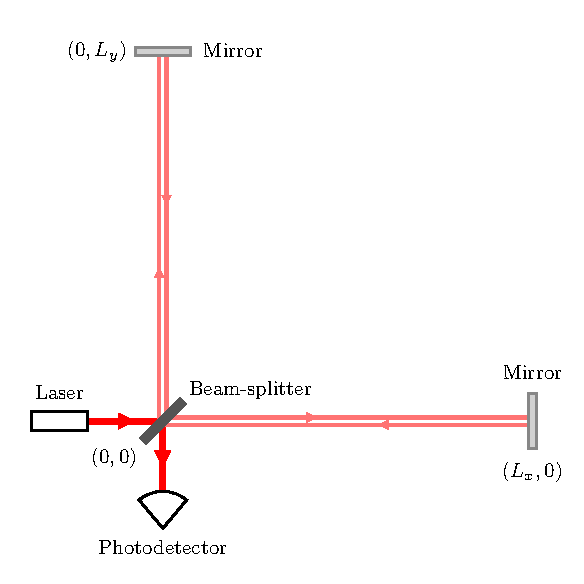
\includegraphics[width=0.6\columnwidth]{Figures/Introduction/interferometer.pdf}
    \caption[Schematic diagram of an interferometer]{ 
    A simple representation of an interferometer, such as those used by LIGO and Virgo to detect GWs. Light from a laser is separated by a beam-splitter and travels down the two interferometer arms. Mirrors at the end of the arms (which are isolated from the environment and act as test masses) reflect the light, before it is recombined at the beam-splitter and sent to a photodetector.
    }
    \label{ch1:fig:interferometer}
\end{figure}

Being metric perturbations, GWs themselves are not scalar quantities but tensors ($h$ is merely the measurement we make when GWs are ``projected'' onto the interferometer).
GWs are described by two dimensionless amplitudes, $h_+$ and $h_\times$, which are the ``plus'' and ``cross'' polarisations respectively.
These two polarisations, which represent small perturbations to a flat background metric, are encapsulated in the GW strain tensor, $h_{ij}$.
To understand the response of an interferometer to incoming GWs, consider a setup (depicted in Fig.~\ref{ch1:fig:interferometer}) where the interferometer arms are aligned with the $x$- and $y$-axes such that the beam-splitter is at the origin and the mirrors are at the coordinates $(L_x,0)$ and $(0,L_y)$.
Incident GWs will influence the propagation of light in the interferometer arms. 
In the proper detector frame, the GW acts to displace the mirrors. 
This is an intuitive picture, and the response of the mirrors to the passing GWs can be described in terms of Newtonian forces. 
However, GWs take on a very simple form (and become easier to work with) when working in the transverse-traceless (TT) frame.
In this description coordinates are defined by freely-falling masses, meaning the interferometer mirrors do not move under the influence of passing GWs. 
Instead, the propagation of the light in the interferometer arms is modified via the GWs influence on the space-time interval.
In the simple case of a GW with only plus polarisation incoming from the positive $z$-direction (i.e.\, into the page in Fig.~\ref{ch1:fig:interferometer}), the space-time interval becomes
\begin{equation}
    \dd{s}^2 = -c^2 \dd{t}^2 + \qty[1 + h_+(t)] \dd{x}^2 + \qty[1 - h_+(t)] \dd{y}^2 + \dd{z}^2,
\end{equation}
where $h_+(t)$ is the GW amplitude.
Light (here, the laser in the interferometer arms) follows null geodesics, $\dd{s}^2 = 0$, so for the light propagation in the $x$-arm we can write
\begin{equation}
    \dd{x} = \pm c\dd{t} \qty[1 + h_+(t)]^{-1/2} \approx \pm c\dd{t} \qty[1 - \frac{1}{2} h_+(t)]
\end{equation}
for small $h_+$ (as is the case in practice, see Eq.~\ref{ch1:eq:quadrupole_strain_oom}).
The plus sign corresponds to light travelling from the beam-splitter to the mirror in the positive $x$-direction; integrating along the length of the arm (where $t_0$ is the time the light leaves the beam-splitter and $t_1$ is the arrival time at the mirror) we have
\begin{gather}
    \int_0^{L_x} \dd{x} = \int_{t_0}^{t_1} c\dd{t} \qty[1 - \frac{1}{2} h_+(t)] \\
    \implies L_x = c(t_1 - t_0) - \frac{c}{2} \int_{t_0}^{t_1} \dd{t} h_+(t). \label{ch1:eq:lx_outward}
\end{gather}
Similarly, for the return trip we have
\begin{equation}\label{ch1:eq:lx_return}
    L_x = c(t_2 - t_1) - \frac{c}{2} \int_{t_1}^{t_2} \dd{t} h_+(t),
\end{equation}
where $t_2$ is the arrival time back at the beam-splitter.
Summing Eqs.~\ref{ch1:eq:lx_outward} and \ref{ch1:eq:lx_return} we obtain
\begin{equation}
    T_x = t_2 - t_0 = \frac{2L_x}{c} + \frac{1}{2}\int_{t_0}^{t_2} \dd{t} h_+(t),
\end{equation}
so the GW acts to modify the usual round-trip travel time of $2L_x/c$.
If we set $h_+(t) = h$ (that is, if we consider a GW of constant amplitude), we can write
\begin{equation}
    T_x = \frac{2L_x}{c}\qty(1-\frac{1}{2}h)^{-1} \approx \frac{2L_x}{c}\qty(1+\frac{1}{2}h).
\end{equation}
Repeating the above for the $y$-arm, we obtain
\begin{equation}
    T_y = \frac{2L_y}{c}\qty(1-\frac{1}{2}h).
\end{equation}
Since the GW alters the round-trip time in the $y$-arm differently, light that left the photodetector initially in-phase will arrive back at the photodetector out of phase.
Setting $L_x = L_y = L$, we can write the difference in arrival time as
\begin{equation}
    \Delta T = T_x - T_y = \frac{2L}{c}h \implies \Delta \phi = \omega \Delta T = \frac{2\omega L}{c}h
\end{equation}
where $\omega$ is the light angular frequency. 
This difference in phase, $\Delta\phi$, is how the GW influences the power measured at the photodetector. 

Einstein~\cite{Einstein:1918btx} showed the GW emission from slowly changing and weakly gravitating sources is quadrupolar to leading order, and far from the source the GW strain tensor can be written
\begin{equation}\label{ch1:eq:quadrupole_strain}
    h_{ij} = \frac{2G}{c^4 r}\ddot{Q}_{ij}.
\end{equation}
Here, $r$ is the distance to the source, and $Q_{ij}$ is the traceless mass quadrupole of the source:
\begin{equation}\label{ch1:eq:quadrupole}
    Q_{ij} = \int \dd[3]{\vb*{x}} \rho(\vb*{x}) \qty(x_i x_j - \frac{1}{3} \abs{\vb*{x}} \delta_{ij}),
\end{equation}
were $\rho(\vb*{x})$ is the mass density and we have used Cartesian coordinates $\vb*{x} = (x_1, x_2, x_3) = (x,y,z)$ with some suitable choice of origin.
Note that the above is valid when $h_{ij}$ is chosen to be in the TT gauge.

It was also shown that the GW luminosity is given by
\begin{equation}\label{ch1:eq:gw_luminosity}
    \dot{E}_\mathrm{GW} = \frac{G}{5c^5} \bigl \langle \dddot{Q}_{ij} \dddot{Q}^{ij} \bigr \rangle,
\end{equation}
where the average (denoted by the angled brackets) is to be taken over $\sim$ a few GW wavelengths.

To perform some simple order-of-magnitude calculations we can introduce a characteristic mass, length and timescale of the radiating system: $M$, $R$, and $T$ respectively.
Starting with the GW luminosity, from dimensional arguments we approximate the quadrupole moment as 
\begin{equation}
    \dddot{Q} \sim \frac{MR^2}{T^3} \sim \frac{Mv^3}{R}
\end{equation}
where $v$ is the characteristic velocity of the system.
Substituting into Eq.~\ref{ch1:eq:gw_luminosity}, we can express the order-of-magnitude GW luminosity as
\begin{equation}\label{ch1:eq:gw_luminosity_oom}
    \dot{E}_\mathrm{GW} \sim \frac{G}{5c^5} \qty(\frac{Mv^3}{R})^2 \sim \frac{c^5}{G} \qty(\frac{r_s}{R})^2 \qty(\frac{v}{c})^6
\end{equation}
where $r_s = 2GM/c^2$ is the Schwarzschild radius (note that we have dropped all constants of order 1 in Eq.~\ref{ch1:eq:gw_luminosity_oom}).
From Eq.~\ref{ch1:eq:gw_luminosity_oom} we immediately see that to maximise energy radiated as GWs we need compact ($R \sim r_s$) and relativistic ($v \sim c$) systems.
Of course, we also need a time-varying quadrupole (Eq.~\ref{ch1:eq:quadrupole_strain}); the mergers of compact objects, then, make ideal systems.
We can similarly obtain the order-of-magnitude GW strain. 
Assuming that our source is indeed a binary system, we can use Kepler's third law to relate the characteristic length scale and frequency $f = 1/T$:
\begin{equation}
    R^3 \sim \frac{GM}{f^2}.
\end{equation}
Our expression for the strain, Eq.~\ref{ch1:eq:quadrupole_strain}, then becomes
\begin{equation}
    h \sim \frac{G}{c^4 r} \frac{MR^2}{T^2} \sim \frac{(GM)^{5/3}f^{2/3}}{c^4 r}.
\end{equation}
The first GW event, GW150914, occurred roughly $440\,\mathrm{Mpc}$ from Earth and had a total binary mass of $72\,M_\odot$.
And, as we will see, current GW detectors are most sensitive to frequencies $\sim 100\,\mathrm{Hz}$.
Expressing the GW strain in terms of these numbers gives
\begin{equation}\label{ch1:eq:quadrupole_strain_oom}
    h \sim 10^{-21} \qty(\frac{M}{72\,M_\odot})^{5/3} \qty(\frac{f}{100\,\mathrm{Hz}})^{2/3} \qty(\frac{440\,\mathrm{Mpc}}{r}),
\end{equation}
emphasising the just how sensitive the interferometers need to be.

Going beyond these simple calculations, it is well-understood how the dynamics of compact-object mergers translate to the measured strain, which allows us to learn about the signal origin.
The GW signal from a BBH merger can be split into three stages: the inspiral, merger, and ringdown.
The inspiral corresponds to the two BHs in the binary orbiting each other. 
Unlike in the Newtonian case, the generation of GWs causes the system to lose energy (Eq.~\ref{ch1:eq:gw_luminosity}) and for the orbit to shrink and spiral. 
This stage in the binary evolution, where the motion of the orbit is slow compared to the speed of light, can be modelled with corrections to the Newtonian case in a post-Newtonian framework~\cite{Blanchet:2013haa}. 
Eventually, the BHs come together in the highly energetic and dynamical merger; this process requires the full nonlinear equations of GR, and is the subject of numerical relativity (NR)~\cite{Duez:2018jaf}. 
Immediately after merging, the final BH is highly distorted. 
As it equilibrates it produces GWs which roughly take the form of a damped sinusoid. 
This is analogous to the ringing a bell makes after it has been struck, and this final stage is called the ringdown.
Just as the early inspiral can be studied by considering deviations to a Newtonian system, the ringdown can be studied by considering perturbations to a static BH spacetime~\cite{Sasaki:2003xr, Pound:2021qin}. 
It is not known beforehand when this perturbative treatment of the final BH becomes valid (i.e., when the ringdown actually starts), and so care must be taken; this will be a recurring theme throughout this work.

\begin{figure}
    \centering
    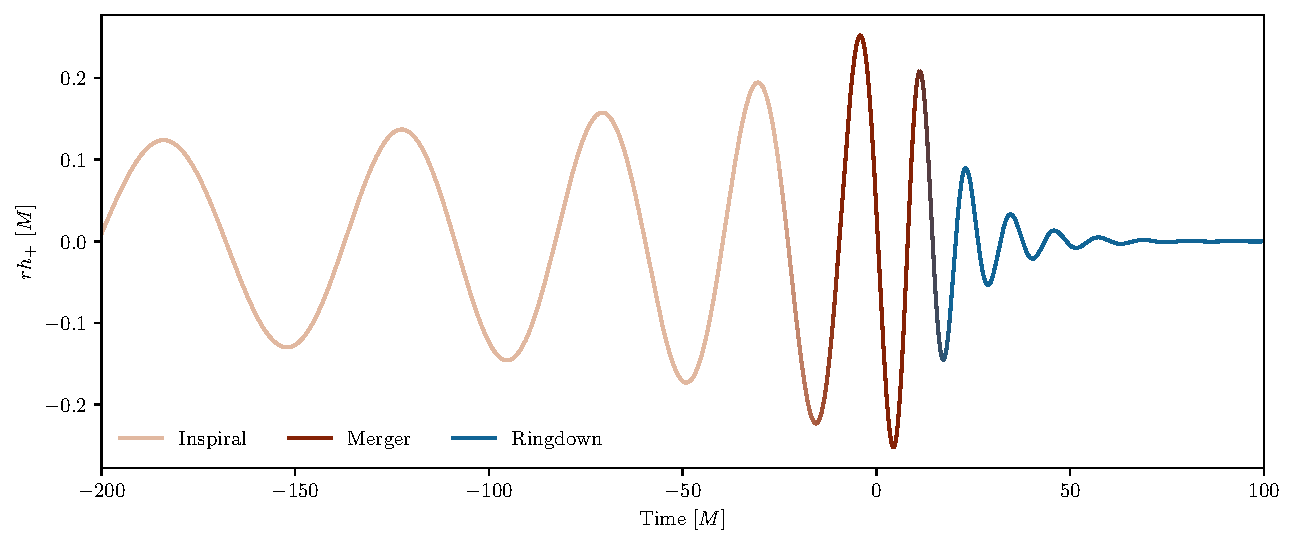
\includegraphics[width=0.9\columnwidth]{Introduction/td_waveform.pdf}
    \caption[Time-domain gravitational-wave signal from a binary black-hole merger]{ 
    The GW signal from a BBH merger. 
    This waveform was generated using the NRSur7dq4 surrogate, and projected onto the Hanford detector using parameters consistent with GW150914 (this includes choosing a sky location and polarisation angle).
    }
    \label{ch1:fig:td_waveform}
\end{figure}

The GW signal from these three stages is shown in Fig.~\ref{ch1:fig:td_waveform}.
Plotted is the (noiseless) GW strain signal projected onto the LIGO Hanford detector, $h$, multiplied by the distance to the source, $r$, as a function of time. 
We use geometric units ($G = c = 1$) to express these quantities in units of the total binary mass, $M$. 
In geometric units we can convert between lengths, masses, and times with appropriate combinations of $G$ and $c$; this means $\mathrm{time}/M$ and $rh/M$ can be made dimensionless quantities. 
Using GW150914 again as an example, say we had a system with total mass $M = 72\,M_\odot \approx 1.43 \times 10^{32}\,\mathrm{kg}$ at a distance $r = 440\,\mathrm{Mpc} \approx 1.36 \times 10^{25}\,\mathrm{m}$. 
Expressing $M$ in seconds gives us the conversion factor for time:
\begin{equation}
    M \times \frac{G}{c^3} \approx 1.43 \times 10^{32}\, \mathrm{kg} \times \frac{6.67 \times 10^{-11}\, \mathrm{m}^3\, \mathrm{kg}^{-1}\, \mathrm{s}^{-2}}{\qty(3 \times 10^8\, \mathrm{m}\, \mathrm{s}^{-1})^3} \approx 3.6 \times 10^{-4}\, \mathrm{s}.
\end{equation}
So, for these system properties, in Fig.~\ref{ch1:fig:td_waveform} we have a ringdown duration of $\sim 50\,M \approx 50 \times 3.6 \times 10^{-4}\,\mathrm{s} \approx 0.018\,\mathrm{s}$. 
Calculating the dimensionless quantity $M/r$ gives us the conversion for the GW amplitude. 
One way to do this is to express $r$ in seconds by dividing by $c$, then use our previous result for $M$:
\begin{equation}
    \frac{M \times G/c^3}{r/c} \approx \frac{3.6 \times 10^{-4}\,\mathrm{s}}{1.36 \times 10^{25}\, \mathrm{m}/3 \times 10^8\, \mathrm{m}\, \mathrm{s}^{-1}} \approx 7.85 \times 10^{-21}.
\end{equation}
This gives a peak strain amplitude in Fig.~\ref{ch1:fig:td_waveform} of $\sim 0.2 \times 7.85 \times 10^{-21} \approx 1.60 \times 10^{-21}$, in agreement with our order-of-magnitude calculation in Eq.~\ref{ch1:eq:quadrupole_strain_oom}. 
This can also be compared with what was actually measured for GW150914 (see Fig.~1 in Ref.~\cite{LIGOScientific:2016aoc}), and we see these numbers are consistent.

The waveform was generated using the NRSur7dq4~\cite{Varma:2019csw} surrogate waveform with zero spins, equal mass ratio, and zero inclination. 
Surrogates effectively ``interpolate'' the waveforms from full NR simulations, allowing quick waveform generation for any choice of system parameters (within the validity of the model). 
For NRSur7dq4 the simulations used to build the model came from the SXS catalog~\cite{Boyle:2019kee}, which we use extensively in Chapter~\ref{Chapter2}. 
Along with the intrinsic system parameters, to project onto the Hanford detector we also choose an event time, sky location and polarisation angle consistent with GW150914.

The above discussion disregards the sensitivity of the detector to different frequencies (i.e.\ the detector noise).
It is standard to treat the noise in the LIGO and Virgo detectors as stationary and Gaussian~\cite{LIGOScientific:2019hgc}.
Stationarity means that the noise covariance matrix is diagonal in the frequency domain (meaning there is no correlation between frequency bins), and so we can describe the noise with a power spectral density (PSD) $S_n(f)$.
In each frequency bin we model the noise as having a random phase and an amplitude drawn from a Gaussian distribution with standard deviation $\sqrt{S_n(f)}$.
\begin{figure}
    \centering
    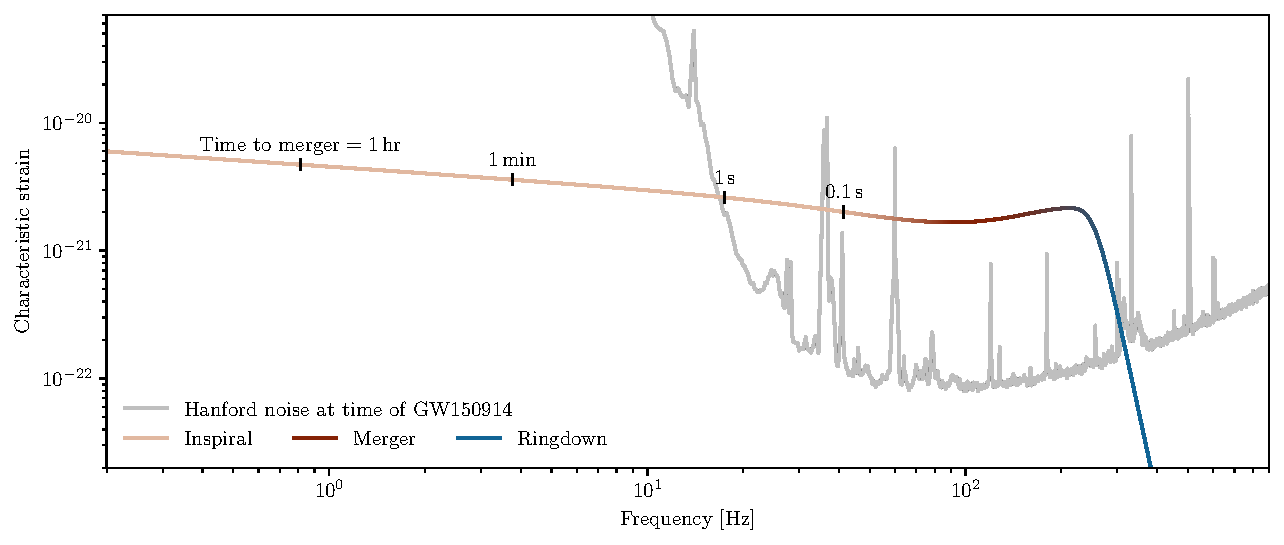
\includegraphics[width=0.9\columnwidth]{Introduction/fd_waveform.pdf}
    \caption[Frequency-domain gravitational-wave signal from a binary black-hole merger]{ 
    The frequency-domain GW signal from a BBH merger, shown with the Hanford sensitivity curve (both expressed through the characteristic strain). 
    The signal was generated with \textsc{IMRPhenomD} using parameters consistent with GW150914.
    }
    \label{ch1:fig:fd_waveform}
\end{figure}
We show the Hanford PSD in Fig.~\ref{ch1:fig:fd_waveform}, along with a frequency-domain BBH GW signal (both expressed through the characteristic strain, see Eqs.~\ref{ch1:eq:hn} and \ref{ch1:eq:hn}).
Since we are now comparing with a PSD, we fix the BBH total mass and distance to the example numbers used above ($M = 72\,M_\odot$, $r = 440\,\mathrm{Mpc}$).
Roughly speaking, the GW signal from a BBH merger increases in frequency over time.
The majority of the inspiral signal is at too low a frequency to be detected, with the GW signal only entering the detector band ($\sim 20$ to $\sim 1000\,\mathrm{Hz}$) just before merger.
Although the binary can spend billions of years inspiralling, we observe only the last few tenths of a second of the merger.
We choose to plot the signal and noise curve in terms of the characteristic strain~\cite{Moore:2014lga}, given by
\begin{equation}\label{ch1:eq:hc}
    h_c(f) = 2f\abs{\tilde{h}(f)}
\end{equation}
for the GW signal (where $\tilde{h}$ is the frequency-domain GW in a given detector), and
\begin{equation}\label{ch1:eq:hn}
    h_n(f) = \sqrt{fS_n(f)}
\end{equation}
for the noise curve.
The characteristic strain has the property that the signal-to-noise ratio (SNR) $\rho$ is given by
\begin{equation}
    \rho^2 = \int_{-\infty}^\infty \dd{\log{f}} \qty[\frac{h_c(f)}{h_n(f)}]^2.
\end{equation}
Evaluating for the above figure we get $\rho \sim 17$, which is consistent with the Hanford SNR for GW150914 (assuming equal SNRs in Hanford and Livingston, a network SNR of 26~\cite{LIGOScientific:2021usb} gives a single detector SNR of $\sim 18$).

Also shown in the figure is the time to merger at select frequencies of the inspiral.
This is to emphasise how the frequency of the binary evolves over time, spending the vast majority of its life in the inspiral with a slowly shrinking orbit.
The leading-order time to merger, $\tau_\mathrm{merge}$, as a function of GW frequency is given by
\begin{equation}\label{ch1:eq:time_to_merger}
    \tau_\mathrm{merge} = \frac{5}{256} \qty(\pi f)^{-\frac{8}{3}} \qty(\frac{G\mathcal{M}}{c^3})^{-\frac{5}{3}},
\end{equation}
where $\mathcal{M}$ is a combination of the two masses in the binary known as the chirp mass,
\begin{equation}
    \mathcal{M} = \frac{(m_1 m_2)^{3/5}}{(m_1 + m_2)^{1/5}}.
\end{equation}
For GW150914, we have $m_1 = 39\,M_\odot$ and $m_2 = 33\,M_\odot$.
In Eq.~\ref{ch1:eq:time_to_merger} we also explicitly show the factors of $G$ and $c$ for clarity (in geometric units these would be set to 1, and it would be implied that the chirp mass should be expressed in units of time). 
This expression for the time to merger is valid in the quasi-circular orbit regime; it can be derived by equating the time derivative of the orbital energy of a binary system to (negative) the GW luminosity (Eq.~\ref{ch1:eq:gw_luminosity}), where the quadrupolar moment is most easily calculated using the equivalent one-body problem with a reduced mass.

The signal in Fig.~\ref{ch1:fig:fd_waveform} was generated with the \textsc{IMRPhenomD}~\cite{Khan:2015jqa} waveform model, as implemented in the \textsc{ripple}~\cite{Edwards:2023sak} Python package.
Phenom models produce approximate waveforms using closed-form analytic expressions in the frequency-domain, making evaluation quick and suitable for GW searches and parameter estimation.
The Hanford PSD is estimated from $1024\,\mathrm{s}$ of off-source data at the time of GW150914 using a Welch periodogram~\cite{1161901}.


\section{Black-hole ringdown}
\label{ch1:sec:bh_ringdown}

\begin{figure}[t!]
    \centering
    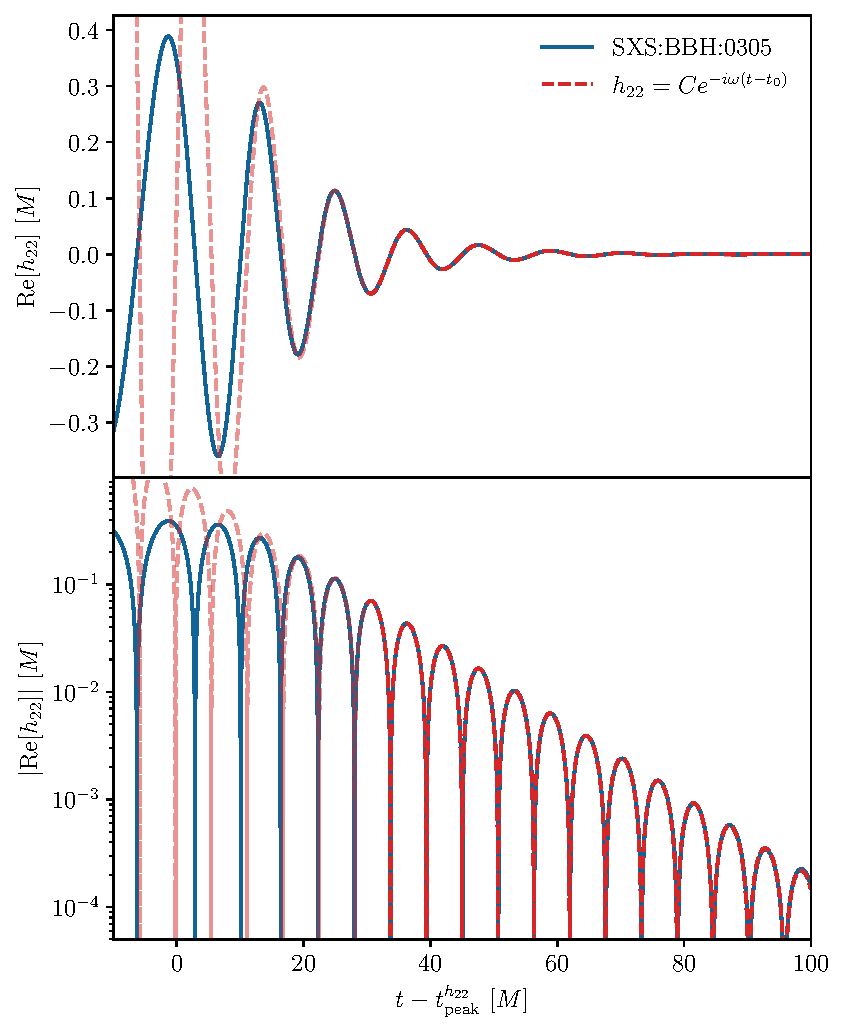
\includegraphics[width=0.6\columnwidth]{Introduction/ringdown_waveform.pdf}
    \caption[Gravitational-wave ringdown waveform]{ 
    The ringdown waveform from a BBH, fitted with a simple damped sinusoid. 
    At early times this simple description breaks down. 
    The waveform is a NR simulation from the SXS catalog.
    }
    \label{ch1:fig:rd_waveform}
\end{figure}

The endpoint of a BBH, the ringdown signal is produced by the remnant BH settling to its stationary state.
Just as a bell or drum has a characteristic sound, so too does a BH; associated with the BH is a unique spectrum of oscillatory modes, determined purely by its properties (namely, for astrophysical BHs, a mass and spin).
The characteristic oscillations of the remnant BH are called quasinormal modes (QNMs), so-called because, unlike normal modes, they decay over time (for reviews on the subject, see Refs.~\cite{Kokkotas:1999bd, Nollert:1999ji, Ferrari:2007dd, Berti:2009kk}).
The QNM frequencies are complex, $\omega = 2\pi f - i/\tau$, with the real part $f$ giving the oscillation frequency and the reciprocal of the imaginary part $\tau$ giving the damping time. 
The QNM spectrum is the subject of Sections~\ref{ch1:sec:qnms} and \ref{ch1:sec:bh_spectroscopy}.
The ringdown signal consists of a sum of QNMs, each excited a different amount depending on the initial configuration of the binary and how they merged; the excitation of different ringdown modes is among the areas of investigation in Chapter~\ref{Chapter2}.

Fig.~\ref{ch1:fig:rd_waveform} shows (in blue) the ringdown portion of the waveform from a NR simulation, SXS:BBH:0305~\cite{Lovelace:2016uwp}.
This simulation has properties consistent with GW150914, and will be among the NR simulations studied in Chapter~\ref{Chapter2}.
NR waveforms are decomposed into spherical-harmonic modes indexed by $\ell$ and $m$ (see Section~\ref{ch2:sec:model} and Eq.~\ref{ch2:eq:spherical_expansion} for more details), and here we plot the real part of the dominant $\ell = m = 2$ mode.
The radial dependence of GW waveforms goes predominantly as $r^{-1}$, so the SXS catalog provides the strain multiplied by $r$ (just as what was plotted in Fig.~\ref{ch1:fig:td_waveform}).
For clarity, when dealing with NR simulations (as we do throughout Chapter~\ref{Chapter2}), we will drop the $r$ factor and have the $r^{-1}$ scaling implied.

Overplotted is a simple model for the $h_{22}$ mode: a exponentially damped sinusoid with complex frequency $\omega = 2\pi f - i/\tau$ and amplitude $C = Ae^{i\phi}$. 
Taking the real part we have
\begin{align}
    \Re[Ce^{-i\omega(t-t_0)}] = A\cos[2\pi f(t-t_0) - \phi]e^{-(t-t_0)/\tau}.
\end{align}
That such a simple model describes the final stages of such a complicated system is a remarkable result, and is part of the power of studying the ringdown.
A faded red line traces the damped sinusoid to earlier times, where it starts to lose validity.
This is to be expected: at earlier times we approach the nonlinear and strong-gravity merger, where BH perturbation theory (which is where this simple damped-sinusoid description comes from) starts to break down.
Note, however, that our model here only includes a single term (i.e., one ringdown QNM); with additional QNMs we may be able to get a better fit to the NR waveform, or to describe the waveform at earlier times (this idea is explored at length in Chapter~\ref{Chapter2}).
A particular subset of QNMs, known as ``overtones'', will be of particular interest throughout the thesis; as well as featuring in the numerical studies of Chapter~\ref{Chapter2}, they will be a target in the analysis of GW data in Chapters~\ref{Chapter3} and \ref{Chapter4}.

A key goal in GW astronomy is the identification of QNMs in the ringdown signal.
We will see in the following sections that QNMs carry information about the remnant BH, meaning that measurements of QNM frequencies give us a way of inferring the remnant BH properties independently of the rest of the GW signal.
This forms the basis of important tests of GR, and is discussed further in Section~\ref{ch1:sec:bh_spectroscopy}.
The testing-GR companion papers for the second~\cite{LIGOScientific:2020tif} and third~\cite{LIGOScientific:2021sio} GW event catalogs featured searches for QNMs; of the detected events, results were reported for 22.
This can be taken as a rough guide for how many events have at least one measurable ringdown mode.
On top of this, tentative evidence was reported for the identification of an additional ringdown mode in a few of the loudest events, including GW150914.
However, as will be seen, the identification of subdominant ringdown modes is subtle.
This is particularly true for one of the most massive BBH mergers observed so far, GW190521~\cite{LIGOScientific:2020iuh}, which has a total source frame mass of $\sim 150\,M_\odot$.
Its large mass means this event enters the detector band only very near merger, and so is ringdown dominated.
This makes it a promising target for QNM searches, and along with GW150914 it is an event that will be referenced throughout this thesis. 

\section{Quasinormal modes}
\label{ch1:sec:qnms}

The characteristic vibrational modes of dissipative systems are known as QNMs.
As stated above, these differ from usual normal modes because they decay over time.
Although not limited to BHs (any real-world physical systems which are subject to damping will exhibit decaying modes), BH spacetimes are an interesting case because even idealised systems are intrinsically dissipative. 

Gravitational perturbations of the Schwarzschild geometry~\cite{Schwarzschild:1916uq} were first studied by Regge and Wheeler~\cite{Regge:1957td}, and this work was extended by Zerilli to a more general class of perturbations~\cite{Zerilli:1970se, Zerilli:1970wzz}.
Employing the perturbation techniques developed by Regge and Wheeler, Vishveshwara~\cite{Vishveshwara:1970zz} performed numerical studies involving the scattering of GWs off a Schwarzschild BH.
It was found that the late-time GW waveform consisted of damped sinusoids, the form of which carried information about the BH mass. 
Further numerical work by Press~\cite{Press:1971wr}, studying the evolution of perturbations to the Schwarzschild geometry, identified the damped sinusoids as the ``free oscillation of a black hole''.
This work was also the first instance of describing the vibration of a BH as a ``quasi-normal mode''.

Equations governing the perturbations of the Kerr metric~\cite{Kerr:1963ud} were found by Teukolsky~\cite{Teukolsky:1972my, Teukolsky:1973ha}. 
Describing rotating BHs, these are expected to be the most general class of astrophysical BH and will be the focus throughout this thesis. 
A remnant Kerr BH has ``no hair''~\cite{Carter:1971zc}, meaning it is fully described by only a final mass and an angular momentum (which we will express via a dimensionless spin parameter). 
The same is true of the spectrum of Kerr QNM frequencies, which are also functions of only the mass and spin. 
This is how QNMs carry information about the remnant BH, and this fact forms the basis of the GR tests discussed further in Section~\ref{ch1:sec:bh_spectroscopy}.

The QNM frequencies can be calculated within the framework of linearised gravity, treating the gravitational field in the vicinity of the remnant as a small (linear) perturbation of the Kerr metric.
Therefore, the QNM description of the GW signal is only expected to be valid at sufficiently late times, when the nonlinearities from the merger have largely decayed away. 
In the following subsections we discuss the calculation and physical picture of QNMs further to help build some intuition.

\subsection{Scalar field on a Schwarzschild background}
\label{ch1:sec:scalar}

To help build some intuition regarding the origin of the QNMs, we will perform a demonstrative calculation involving a massless scalar field, $\psi(t,r,\theta,\phi)$, on a Schwarzschild background.
This will lead to equations reminiscent of the Zerilli and Regge-Wheeler equations, without the complication of tensor spherical harmonics that comes with the full gravitational-perturbation treatment.

The metric tensor, in Schwarzschild coordinates, is
\begin{equation}\label{ch1:eq:schwarzschild}
g_{\mu\nu} = \begin{pmatrix}
- \left(1 - \frac{2M}{r}\right) & 0 & 0 & 0 \\
0 & \left(1 - \frac{2M}{r}\right)^{-1} & 0 & 0 \\
0 & 0 & r^2 & 0 \\
0 & 0 & 0 & r^2 \sin^2\theta
\end{pmatrix},
\end{equation}
where now $M$ is the mass of the BH (and not the total mass of the binary, as before). 
The relevant massless wave equation, qualitatively similar to equations describing GWs and electromagnetic waves (and used here as a toy model for the GW perturbations of a BH), is the Klein-Gordon equation 
\begin{equation}
    \nabla_\mu \nabla^\mu \psi = 0.
\end{equation}
Using the fact that a covariant derivative reduces to the partial derivative on scalars, we can write this as
\begin{equation}
    \nabla_\mu \nabla^\mu \psi = \frac{1}{\sqrt{-g}} \partial_\mu \qty(\sqrt{-g} g^{\mu\nu} \partial_\nu \psi) = 0
\end{equation}
where $g$ is the determinant of the metric tensor, $g^{\mu\nu}$ is the inverse of the metric tensor, and we have also used $\Gamma^\mu_{\mu\nu} = \partial_\nu \ln{\sqrt{-g}} = \qty(-g)^{-1/2} \partial_\nu \sqrt{-g}$.
For Schwarzschild we have $\sqrt{-g} = r^2 \sin{\theta}$.
Evaluating, we get
\begin{multline}
    - \qty(1 - \frac{2M}{r})^{-1} \pdv[2]{\psi}{t} + \frac{1}{r^2} \pdv{r} \qty[r^2 \qty(1 - \frac{2M}{r}) \pdv{\psi}{r} ]\\
    + \frac{1}{r^2} \qty[ \frac{1}{\sin{\theta}} \pdv{\theta} \qty(\sin{\theta} \pdv{\psi}{\theta} ) + \frac{1}{\sin^2{\theta}} \pdv[2]{\psi}{\phi} ] = 0.
\end{multline}
Recognising that the scalar spherical harmonics, $Y_{\ell m}(\theta,\phi)$, are the eigenfunctions of the angular part:
\begin{equation}\label{ch1:eq:spherical}
    \frac{1}{\sin{\theta}} \pdv{\theta} \qty(\sin{\theta} \pdv{Y_{\ell m}}{\theta} ) + \frac{1}{\sin^2{\theta}} \pdv[2]{Y_{\ell m}}{\phi} = - \ell (\ell + 1) Y_{\ell m},
\end{equation}
we will attempt a spherical-harmonic decomposition of the scalar field. 
With the expectation that the radial dependence of the field will go as $1/r$ (and also anticipating a change in radial coordinate) we write the scalar field as
\begin{equation}\label{ch1:eq:scalar_spherical_expansion}
    \psi(t, r, \theta, \phi) = \frac{1}{r} \sum_{\ell = 0}^\infty \sum_{m = -\ell}^\ell \psi_{\ell m}(t, r) Y_{\ell m}(\theta, \phi).
\end{equation}
Substituting, we are left with an equation for the radial part:
\begin{multline}
    - \pdv[2]{\psi_{\ell m}}{t} + \frac{1}{r} \qty(1 - \frac{2M}{r}) \pdv{r} \qty[r^2 \qty(1 - \frac{2M}{r}) \pdv{r}\qty(\frac{\psi_{\ell m}}{r}) ]\\
    - \qty(1 - \frac{2M}{r}) \qty(\frac{\ell (\ell + 1)}{r^2}) \psi_{\ell m} = 0.
\end{multline}
To proceed we introduce the tortoise coordinate, $r_*$,
\begin{equation}
    r_* = r + 2M \ln(\frac{r}{2M} - 1),
\end{equation}
which has the property that
\begin{equation}
    \dv{r_*}{r} = \qty( 1 - \frac{2M}{r} )^{-1}.
\end{equation}
Note that as $r$ approaches the Schwarzschild radius ($r \rightarrow 2M$), the tortoise coordinate $r_* \rightarrow -\infty$.
Making this change of variables, we arrive at
\begin{equation}\label{ch1:eq:wave_equation}
    \pdv[2]{\psi_{\ell m}(t,r)}{r_*} - \pdv[2]{\psi_{\ell m}(t,r)}{t} - V_\ell(r) \psi_{\ell m}(t,r) = 0,
\end{equation}
where
\begin{equation}
    V_\ell(r) = \qty( 1 - \frac{2M}{r} ) \qty( \frac{\ell (\ell + 1)}{r^2} + \frac{2M}{r^3} )
\end{equation}
is an effective potential.
Performing a Fourier transform, 
\begin{equation}\label{ch1:eq:ft}
    \tilde{\psi}_{\ell m}(\omega,r) = \int_{-\infty}^\infty \dd{t} \psi(t,r) e^{-2\pi i f t},
\end{equation}
we can bring Eq.~\ref{ch1:eq:wave_equation} into the form of a one-dimensional Schr\"{o}dinger equation
\begin{equation}\label{ch1:eq:fd_wave_equation}
    \pdv[2]{\tilde{\psi}_{\ell m}(\omega,r)}{r_*} + \qty[ \omega^2 - V_\ell(r)] \tilde{\psi}_{\ell m}(\omega,r) = 0.
\end{equation}
Gravitational perturbations obey an equation of the same form (i.e. the Regge-Wheeler and Zerilli equations), and in fact the effective potential can be written in the unified form
\begin{equation}\label{ch1:eq:rw_potential}
    V_\ell(r) = \qty( 1 - \frac{2M}{r} ) \qty( \frac{\ell (\ell + 1)}{r^2} + \frac{(1 - s^2)2M}{r^3} )
\end{equation}
with $s = 0$, $-1$ and $-2$ for scalar, electrical, and gravitational perturbations respectively. 
We plot $V_\ell(r)$ in Fig.~\ref{ch1:fig:rw_potential} for the scalar and gravitational perturbation cases, and for a few different values of $\ell$. 
Note that the minimum value of $\ell$ permitted is given by $\abs{s}$.

\begin{figure}[t]
    \centering
    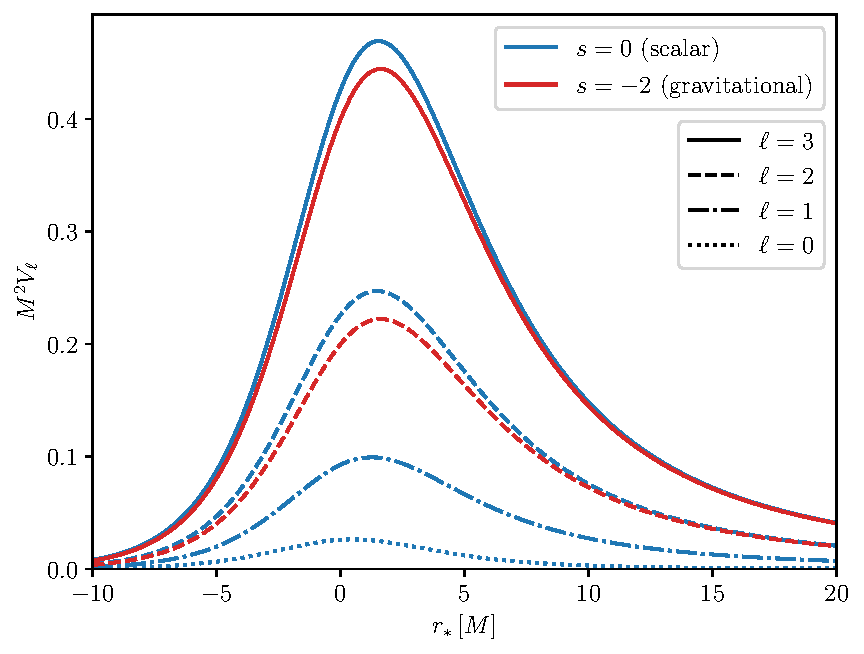
\includegraphics[width=0.6\columnwidth]{Figures/Introduction/rw_potential.pdf}
    \caption[Regge-Wheeler potential]{
    The Regge-Wheeler potential as a function of the tortoise coordinate $r_*$ (with the BH horizon at $r_* = -\infty$), for scalar and gravitational perturbations and for a selection of $\ell$. In this subsection $M$ refers to the mass of the Schwarzschild BH, and not the total binary mass.
    }
    \label{ch1:fig:rw_potential}
\end{figure}

When studying gravitational perturbations, we write the metric as
\begin{equation}
    g'_{\mu\nu} = g_{\mu\nu} + h_{\mu\nu},
\end{equation}
where $g_{\mu\nu}$ is the unperturbed BH spacetime (i.e., for Schwarzschild, Eq.~\ref{ch1:eq:schwarzschild}) and $h_{\mu\nu}$ is a perturbation. 
An analogous procedure to the above is followed, and it is worth noting that the angular dependence is now described by spin-weighted functions that are generalisations of the usual spherical harmonics.
In the case of Schwarzschild, these are the spin-weighted spherical harmonics, ${}_sY_{\ell m}(\theta,\phi)$.
These are also the functions commonly used as the basis in the expansion of NR waveforms; see the discussion around Eq.~\ref{ch2:eq:spherical_expansion} for more details.
Spin-weighted functions differ from their usual scalar counterparts via their transformation properties, see Sec.~\ref{misaligned-spin-section} for more details.
In the case of Kerr, a set of functions called the spin-weighted spheroidal harmonics, ${}_{s}S_{\ell m}(\theta, \phi; \gamma)$ are required~\cite{Teukolsky:1973ha}.
The quantity $\gamma$ is called the spheroidicity or oblateness, and it depends on the BH spin (see the discussion around Eq.~\ref{ch2:eq:spheroidal_expansion} for more details).
The spheroidal harmonics are solutions of the equation
\begin{equation}\label{ch1:eq:spheroidal}
    \qty[\frac{1}{\sin{\theta}} \pdv{\theta} \qty(\sin{\theta} \pdv{\theta} ) - \frac{(m + s\cos{\theta})^2}{\sin^2{\theta}} + (\gamma\cos{\theta} - s)^2 - s(s-1) + {}_sA_{\ell m}] {}_{s}S_{\ell m}  = 0,
\end{equation}
where ${}_sA_{\ell m}(\gamma)$ is known as the angular separation constant.
In the limit $\gamma \rightarrow 0$ (corresponding to the Schwarzschild limit), the solutions to Eq.~\ref{ch1:eq:spheroidal} are the spin-weighted spherical harmonics and we have
\begin{equation}
    {}_sA_{\ell m} = \ell(\ell + 1) - s(s + 1).
\end{equation}
If we then set $s = 0$, we recover Eq.~\ref{ch1:eq:spherical} (since we have a $\phi$-dependence of the form $e^{im\phi}$) and the solutions become the normal spherical harmonics.

Returning to the effective potential, Eq.~\ref{ch1:eq:rw_potential}, we note that the Zerilli equation has a slightly different form (the Zerilli equation describes polar, or even-parity, perturbations, whereas the Regge-Wheeler equations describes axial, or odd-parity, perturbations). 
However, it has been shown that the QNM spectrum resulting from the Regge-Wheeler and Zerilli equations are identical~\cite{Chandrasekhar:1975nkd}.

Given Eq.~\ref{ch1:eq:fd_wave_equation} and the effective potential, we must specify boundary conditions to find the QNM solutions.
When solving for the normal modes on a string, or the energy levels of a quantum harmonic oscillator, we require the wavefunction to vanish at the boundaries (either at the string ends, or at $\pm \infty$ for the harmonic oscillator).
The problem we're considering here is slightly different; the potential, depicted in Fig.~\ref{ch1:fig:rw_potential}, clearly does not admit bound states. 
It does not have any minima, and $V_\ell(r) > 0$ for all $r$.
The implication is that we should look for plane wave solutions that are ingoing to the BH horizon, and outgoing to infinity:
\begin{alignat}{2}
    &\tilde{\psi}_{\ell m}(\omega, r) \sim e^{i \omega r_*} \qquad &&\qty(r_* \rightarrow -\infty) \nonumber \\
    &\tilde{\psi}_{\ell m}(\omega, r) \sim e^{- i \omega r_*} \qquad &&\qty(r_* \rightarrow \infty).
\end{alignat}
This follows from the consideration that the field should radiate only inward at the horizon and only outward at spatial infinity.

This gives us a well-posed problem, and now all that is left is the computation of the QNMs. 
A variety of methods have been used~\cite{Kokkotas:1999bd, Berti:2004md}, with the first attempts consisting of the aforementioned time-domain evolutions of the Regge-Wheeler and Zerilli equations by Vishveshwara~\cite{Vishveshwara:1970zz} and Press~\cite{Press:1971wr}. 
In principle the QNM frequencies can be extracted from the resulting waveform, but this approach does not return the complete spectrum (in practice only a subset of modes can be extracted).
Chandrasekhar and Detweiler~\cite{Chandrasekhar:1975zza} employed a shooting method to directly integrate the wave equation in the frequency domain; this involves picking a value for the QNM frequency, integrating, and checking whether the boundary conditions are satisfied. 
This is an inefficient way of identifying QNMs, and this approach is also prone to numerical noise.
Analytical methods were developed by Blome, Mashhoon and Ferrari~\cite{BLOME1984231, Ferrari:1984ozr, Ferrari:1984zz}, which consider the bound states of the inverted BH potential. 
Although not in general accurate, this approach offers physical insight which we touch upon in the next subsection.
Motivated by the analogy between Eq.~\ref{ch1:eq:fd_wave_equation} and the Schr\"{o}dinger equation, Schutz and Will~\cite{Schutz:1985km} employed WKB methods to calculate a handful of fundamental mode QNM frequencies.
This approach has since been improved upon~\cite{Iyer:1986np, Matyjasek:2017psv, Konoplya:2019hlu}, and can give very accurate results for certain modes (but, again, breaks down in some limits). 
Finally, a numerical method utilising continued fractions (proposed by Leaver~\cite{Leaver:1985ax}, and later improved upon by Nollert~\cite{Nollert:1993zz}) is known to be highly accurate and fast.
It is the method of choice in modern codes such as the \textsc{qnm} Python package~\cite{Stein:2019mop} (which is used in work throughout this thesis).
The \textsc{qnm} package actually employs a spectral method, developed in Ref.~\cite{Cook:2014cta}, alongside Leaver's method to solve for the QNM frequencies and angular separation constants. 
In brief, when a separation of variables (similar to Eq.~\ref{ch1:eq:scalar_spherical_expansion}, but with spin-weighted spheroidal harmonics) is applied to the equation governing perturbations to the Kerr metric we obtain coupled radial and angular equations (the Teukolsky equations). 
The \textsc{qnm} package uses Leaver's method to solve the radial equation, but the solutions for the angular equation (the spin-weighted spheroidal harmonics) are expanded in the basis of the spin-weighted spherical harmonics as
\begin{equation}
    {}_{s}S_{\ell m}(\theta,\phi;\gamma) = \sum_{\ell'=\ell_\mathrm{min}}^\infty \mu_{\ell'm\ell}(\gamma) ~ {}_{s}Y_{\ell'm}(\theta,\phi),
\end{equation}
where $\ell_\mathrm{min} = \mathrm{max}(\abs{m},\abs{s})$.
The coefficients, $\mu_{\ell'm\ell}(\gamma)$, are the spherical-spheroidal mixing coefficients~\cite{Berti:2014fga} and will become important when modelling NR data (which is decomposed into spin-weighted spherical harmonics) as a sum of QNMs (whose natural basis is the spin-weighted spheroidal harmonics); see Section~\ref{ch2:sec:fitting} for more details.
When the spheroidal harmonics are expanded in this way (and the upper limit on the sum is replaced by some finite $\ell_\mathrm{max}$), the angular equation becomes an eigenvalue problem with ${}_{s}A_{\ell m}(\gamma)$ as the eigenvalues and $\mu_{\ell'm\ell}(\gamma)$ as the eigenvectors.
So, the spectral approach has the advantage of returning the spherical-spheroidal mixing coefficients as part of the solution.

In summary, when enforcing the above boundary conditions, only discrete values of $\omega$ satisfy Eq.~\ref{ch1:eq:fd_wave_equation}; these are the QNMs.
In the case of a Kerr BH, we denote the QNMs $\omega_{\ell m n}$.
They are indexed by three numbers: the usual angular indices $\ell$ and $m$, and an additional ``overtone'' index $n$.
We present the solutions in Section~\ref{ch1:sec:bh_spectroscopy} and in Fig.~\ref{ch1:fig:qnm_taxonomy}.
The full computation of the spectrum is beyond the scope of this work.
We instead consider a simple calculation of QNMs using the geodesic correspondence in order to build some physical intuition.

\subsection{Quasinormal modes from the geodesic correspondence}
\label{ch1:sec:geodesic}

First pointed out by Goebel~\cite{1972ApJ...172L..95G}, there exists a relation between BH QNMs and null geodesics around the BH spacetime.
Having since been developed further~\cite{BLOME1984231, Ferrari:1984ozr, Ferrari:1984zz, Cardoso:2008bp, Yang:2012he}, this approach provides a physical insight to QNMs; that is, QNMs can be interpreted as GWs slowly leaking out of a light-ring orbit around the BH. 
Although only valid for $\ell \gg 1$ (known as the eikonal, or geometrical optics, limit), this correspondence greatly simplifies the calculations of QNMs since it only depends on the background metric.
Consequently, it offers a way to compute QNMs in beyond GR theories (for example, as was done in Ref.~\cite{Blazquez-Salcedo:2016enn}), or for computing the QNM spectrum for charged (Kerr-Newman~\cite{Newman:1965my}) BHs~\cite{Cardoso:2016olt, Wang:2021uuh} which can be challenging with the previously discussed methods (but, see also Ref.~\cite{Carullo:2021oxn} where a more sophisticated analysis was done).

The key result is that the QNM frequencies for a Kerr BH in the eikonal limit can be written as
\begin{equation}\label{ch1:eq:eikonalomega}
    \omega_{\ell m n} = 2\pi f_{\ell m n} - \frac{i}{\tau_{\ell m n}} = \qty(\ell + \frac{1}{2}) \Omega_\theta + m \Omega_\mathrm{pre} - i \qty(n + \frac{1}{2}) \gamma_L.
\end{equation}
Here, $\Omega_\theta$ is the frequency of small oscillations in the polar direction of a perturbed geodesic. 
The precessional frequency of the orbital plane, $\Omega_\mathrm{pre}$, is given by $\Omega_\mathrm{pre} = \Omega_\phi - \Omega_\theta$, where $\Omega_\phi$ is the orbital frequency of the light ring.
Finally, $\gamma_L$ is the Lyapunov exponent of the light ring; this can be thought of as a measure of the stability of the orbit.
More precisely, it characterises the rate at which the cross section of a congruence of null geodesics on the circular photon orbit increases under radial perturbations.
Crucially, these quantities are all determined by the metric. 
Below we take a the case of a stationary and axisymmetric spacetime (i.e.\ the spacetime associated with a rotating BH) and show how one can calculate the relevant quantities.
For this demonstrative calculation we set $\ell = m$, associated with prograde equatorial motion, to simplify the calculations.
Note that, with the assumption $\ell = m \gg 1$, we can write the real part of the QNM frequency as
\begin{equation}
    \qty(\ell + \frac{1}{2}) \Omega_\theta + m \Omega_\mathrm{pre} \sim \ell \Omega_\theta + \ell \qty(\Omega_\phi - \Omega_\theta) = \ell \Omega_\phi,
\end{equation}
which aligns with the interpretation of QNMs originating as GWs in light ring orbits.

First, we need the metric associated with a stationary and axisymmetric spacetime. 
The stationary and axisymmetric character requires that the metric coefficients be independent of $t$ and $\phi$, so that $g_{\mu \nu} = g_{\mu \nu}(r,\theta)$. 
Note that we haven't imposed equatorial motion ($\theta = \pi/2$) yet.
We also require that the spacetime is invariant to the simultaneous inversion of the time $t$ and the angle $\phi$ (i.e.\ to the transformation $t \rightarrow -t$, $\phi \rightarrow -\phi$). 
This has the physical meaning that the spacetime we are considering is associated with a rotating body. 
This invariance requires 
\begin{equation}
    g_{tr} = g_{t \theta} = g_{\phi r} = g_{\phi \theta} = 0.
\end{equation}
Then we have 
\begin{equation}
	\dd s^2 = g_{tt}\dd t^2 + 2g_{t \phi} \dd t \dd \phi + g_{\phi \phi}\dd \phi^2 + \qty[ g_{rr}\dd r^2 + 2g_{r \theta} \dd r \dd \theta + g_{\theta \theta} \dd \theta^2 ].
\end{equation}
It can be shown~\cite{Chandrasekhar:1985kt} that the term in square brackets can be brought to the diagonal form $g_{r'r'}\dd r'^2 +  g_{\theta' \theta'} \dd \theta'^2$ by a change of coordinates $r'=r'(r,\theta)$ and $\theta'=\theta'(r,\theta)$.
Renaming our variables by removing the primes, this gives
\begin{equation}
    \dd s^2 = g_{tt}\dd t^2 + g_{rr}\dd r^2 + g_{\theta \theta}\dd \theta^2 + g_{\phi \phi}\dd \phi^2 + 2g_{t \phi}\dd t\dd \phi.
\end{equation}
We can find geodesic curves $x^\mu(\lambda)$ by extremising the action $S=\int\mathrm{d}\lambda\,\mathcal{L}$ where the Lagrangian is given by
\begin{align}
    \mathcal{L} &= \frac{1}{2}g_{\mu \nu} \dot{x}^\mu \dot{x}^\nu \\
    &= \frac{1}{2}\qty(g_{tt}\dot{t}^2 + g_{rr}\dot{r}^2 + g_{\theta \theta}\dot{\theta}^2 + g_{\phi \phi}\dot{\phi}^2 + 2g_{t \phi}\dot{t}\dot{\phi}), \nonumber
\end{align}
and a dot denotes a derivative with respect to the affine parameter $\lambda$ along the curve. 
We proceed with the Euler-Lagrange (EL) equations, 
\begin{equation}
    \dv{\lambda}(\pdv{\mathcal{L}}{\dot{x}^\mu}) = \pdv{\mathcal{L}}{x^\mu}.
\end{equation}
Firstly, the stationarity of our spacetime leads to a constant of motion (the energy):
\begin{equation}\label{ch1:eq:el_t} 
    \pdv{\mathcal{L}}{\dot{t}} = -E \implies g_{tt}\dot{t} + g_{t\phi}\dot{\phi} = -E.
\end{equation}
Similarly, from the axisymmetry of the spacetime we have a second constant of motion (the angular momentum):
\begin{equation}\label{ch1:eq:el_phi}
    \pdv{\mathcal{L}}{\dot{\phi}} =L \implies g_{\phi \phi}\dot{\phi} + g_{t\phi}\dot{t} = L.
\end{equation}
From Eqs.~\ref{ch1:eq:el_t} and \ref{ch1:eq:el_phi} we can solve for the two components of the four-velocity $\dot{t}$ and $\dot{\phi}$ to give
\begin{gather}
    \label{ch1:eq:tdot_L}
    \dot{t} = E \frac{g_{\phi \phi} + g_{t \phi}\hat{L}}{\qty(g_{t \phi})^2 - g_{t t}g_{\phi \phi}} \\
    \label{ch1:eq:phidot_L}
    \dot{\phi} = E \frac{g_{t \phi} + g_{t t}\hat{L}}{g_{t t}g_{\phi \phi} - \qty(g_{t \phi})^2}
\end{gather}
where $\hat{L} = L/E$ is the specific angular momentum.
We are also free to rescale our affine parameter $\lambda\rightarrow E\lambda$ to remove $E$ from the above expressions.
Using the above, the azimuthal orbital frequency can be calculated:
\begin{equation}
    \Omega_\phi = \frac{\mathrm{d}\phi}{\mathrm{d}t} =  \frac{\dot{\phi}}{\dot{t}} = -\frac{g_{t\phi}+g_{tt}\hat{L}}{g_{\phi\phi}+g_{t\phi}\hat{L}}.
\end{equation}
In general, for the remaining two coordinates ($r$ and $\theta$) we can use the EL equations to find the second-order differential geodesic equations.
However, now we impose the simplification of equatorial motion mentioned previously: $\theta=\pi/2$.
This implies $\dot{\theta}=0$ in the case of reflective symmetry about the equator. 
This allows us to get a first order equation for $\dot{r}$ by considering the four-velocity for null geodesics:
\begin{equation}\label{ch1:eq:rdot}
    g_{\mu\nu}\dot{x}^\mu\dot{x}^\mu = 0 \implies \dot{r}^2 = V_{\rm eff}(r;\hat{L}),
\end{equation}
where
\begin{align}\label{ch1:eq:veff}
    V_{\rm eff}(r;\hat{L}) &= \frac{-g_{tt}\dot{t}^2 -g_{\phi\phi}\dot{\phi}^2-2g_{t\phi}\dot{t}\dot{\phi} }{g_{rr}} \nonumber \\
    &= \frac{g_{tt} \hat{L}^2+2 g_{t\phi } \hat{L}+g_{\phi\phi}}{g_{rr}(g_{t\phi}^2-g_{tt} g_{\phi \phi})},
\end{align}
and in the final line we have used Eqs.~\ref{ch1:eq:tdot_L} and \ref{ch1:eq:phidot_L} to eliminate $\dot{t}$ and $\dot{\phi}$.
In Eq.~\ref{ch1:eq:veff} the $g_{\mu\nu}$ metric coefficients are to be evaluated on the equatorial plane $\theta=\pi/2$ and so are only functions of $r$.
A light ring is a circular null geodesic orbit. 
The radius, $r_*$, and angular momentum, $\hat{L}_*$, of such an orbit must satisfy $V_{\rm eff} = V'_{\rm eff} = 0$, where a prime denotes a radial derivative with respect to $r$. The first condition yields
\begin{equation}
    \hat{L}_*(r) = \frac{-g_{t \phi} \pm \sqrt{g_{t \phi}^2 - g_{t t}g_{\phi \phi}}}{g_{t t}},
\end{equation}
while the second gives an implicit formula for $r_*$:
\begin{equation}\label{ch1:eq:veffprime}
    V'_{\rm eff}\big(r_*;\hat{L}_*(r_*)\big) = 0.
\end{equation}
In general we solve Eq.~\ref{ch1:eq:veffprime} numerically to obtain the light ring radius.
For prograde equatorial orbits in the Kerr metric this will have a single root, but will depend on the spin chosen for the spacetime.

Having found the equations of the light ring, we now consider neighbouring geodesics (i.e.\ perturbations to the light ring) to determine $\Omega_\theta$ and the Lyapunov exponent. 
First, consider polar motion. 
The EL equation for $\theta$ is 
\begin{equation}\label{ch1:eq:el_theta}
    g_{\theta \theta} \ddot{\theta} + \qty(\pdv{g_{\theta \theta}}{\theta} \dot{\theta} + \pdv{g_{\theta \theta}}{r} \dot{r}) \dot{\theta} = \frac{1}{2} \bigg(\pdv{g_{t t}}{\theta} \dot{t}^2 + \pdv{g_{r r}}{\theta} \dot{r}^2 + \pdv{g_{\theta \theta}}{\theta} \dot{\theta}^2 + \pdv{g_{\phi \phi}}{\theta} \dot{\phi}^2 + 2\pdv{g_{t \phi}}{\theta} \dot{t}\dot{\phi}\bigg).
\end{equation}
We consider small perturbations in the $\theta$ direction about the light ring.
That is, we set $r = r_*$ and $\theta = \pi/2+\delta\theta$.
Discarding terms $\mathcal{O}(\delta\theta^2)$ (and with $\dot{t}$ and $\dot{\phi}$ given by Eqs.~\ref{ch1:eq:tdot_L} and \ref{ch1:eq:phidot_L} respectively) we obtain
\begin{equation}\label{ch1:eq:el_theta_expanded}
    g_{\theta \theta}(r_*,\pi/2) \delta\ddot{\theta} = \frac{1}{2} \bigg(\pdv[2]{g_{t t}(r_*,\pi/2)}{\theta} \dot{t}^2 + \pdv[2]{g_{\phi\phi}(r_*,\pi/2)}{\theta} \dot{\phi}^2 + 2\pdv[2]{g_{t \phi}(r_*,\pi/2)}{\theta} \dot{t}\dot{\phi}\bigg)\delta\theta.
\end{equation}
which describes simple harmonic motion, $\delta\ddot{\theta} = -\tilde{\Omega}^2_\theta \delta\theta$, where the constant $\tilde{\Omega}_\theta$ is the frequency of the oscillations with respect to the parameter $\lambda$.
The frequency of the oscillations with respect to coordinate time $t$ is given by
\begin{align}
    \Omega_\theta = \frac{\tilde{\Omega}_\theta}{\dot{t}} &= \frac{1}{\dot{t}} \sqrt{-\frac{1}{2g_{\theta\theta}}\qty(\pdv[2]{g_{tt}}{\theta}\dot{t}^2 + 2\pdv[2]{g_{t\phi}}{\theta}\dot{t}\dot{\phi} + \pdv[2]{g_{\phi\phi}}{\theta}\dot{\phi}^2)} \nonumber \\
    &= \sqrt{-\frac{1}{2g_{\theta\theta}}\qty(\pdv[2]{g_{tt}}{\theta} + 2\pdv[2]{g_{t\phi}}{\theta}\Omega_\phi + \pdv[2]{g_{\phi\phi}}{\theta}\Omega_\phi^2)},
\end{align}
where all quantities on the right hand side are to be evaluated at the light ring. 
In the case of the Kerr metric $\Omega_\theta^2 > 0$ and the light ring is stable in the polar direction.

Now consider motion in the radial direction ($\dot{r} \neq 0$).
Differentiating Eq.~\ref{ch1:eq:rdot} with respect to $\lambda$ gives
\begin{equation}
    \ddot{r} = \frac{1}{2} \frac{\dot{V}_\mathrm{eff}(r)}{\dot{r}} = \frac{1}{2}V'_\mathrm{eff}(r).
\end{equation}
Consider small perturbations $r = r_* + \delta r$ with $\theta = \pi/2$ and discarding $\mathcal{O}(\delta r^2)$ terms gives
\begin{equation}
    \delta \ddot{r} = \frac{1}{2}V''_{\rm eff}(r_*)\delta r.
\end{equation}
Looking for periodic solutions, the frequency of the radial oscillations (with respect to coordinate time) is given by
\begin{equation}
    \Omega_{r} = \sqrt{-\frac{V''_{\rm eff}(r_*)}{2\dot{t}^2}}.
\end{equation}
In the case of the Kerr metric the light ring orbit has $\Omega_r^2 < 0$ and is unstable in the radial direction; we can define the Lyapunov exponent as
\begin{equation}
    \gamma_L = -i\Omega_r = \sqrt{\frac{V''_\mathrm{eff}(r_*)}{2\dot{t}}}
\end{equation}
and the corresponding decay timescale from Eq.~\ref{ch1:eq:eikonalomega} is
\begin{equation}
    \tau_{\ell m n} = \qty(n + \frac{1}{2})^{-1} \sqrt{\frac{2\dot{t}^2}{V''_\mathrm{eff}(r_*)}}.
\end{equation}
We conclude this section with a discussion of some the problems associated with QNMs.
In Section~\ref{ch1:sec:bh_spectroscopy} we will discuss the full (and accurately computed) QNM spectrum further, and the tests of GR that can be done with the observation of QNMs.

\subsection{Limitations of quasinormal modes}
\label{ch1:sec:limitations}

Although QNMs offer a powerful tool to learn about the remnant BH and test our theories (see Section~\ref{ch1:sec:bh_spectroscopy}), there are some subtleties regarding the QNM spectrum and the ringdown signal that should be pointed out. 

It is known that QNMs, in contrast to normal modes, do not form a complete basis~\cite{Ching:1993gt, Ching:1995rt, Nollert:1998ys, Ching:1998mxl, Nollert:1999ji}, meaning that there are other contributions to the ringdown waveform beyond the QNMs.
In particular, it is known that at late times the ringdown consists of a power-law tail~\cite{Price:1971fb, Leaver:1986gd, Ching:1995tj} (see also Ref.~\cite{Gleiser:2007ti}, and references therein, for a more recent discussion about our knowledge of tails), and nonlinear effects such as GW memory~\cite{Favata:2010zu} may also be present.
Although at a much lower amplitude than the QNM ringing and not resolvable at current detector sensitivities, at sufficient SNRs these effects may need to be considered to avoid biases.
This idea was touched upon in Ref.~\cite{Thrane:2017lqn}, where it was found that their ability to constrain remnant parameters from the ringdown signal actually degraded at high SNRs (late-time tails were suggested as an explanation for this, but it is not clear if they were responsible in this study).
See also Ref.~\cite{Baibhav:2017jhs} for a study on how neglecting these beyond-QNM contributions could bias future studies.

Motivated by work done in Refs.~\cite{Ching:1993gt, Ching:1995rt}, Nollert~\cite{Nollert:1996rf} attempted to make the QNM spectrum complete via modifications to the effective potential (for example, in the case of Schwarzschild, the Regge-Wheeler potential depicted in Fig.~\ref{ch1:fig:rw_potential}).
However, it was found that the QNM spectrum is highly unstable to changes in the potential (no matter how small).
That is, perturbations to the potential (which do not significantly change the physical ringdown waveform) can lead to very different QNM spectra; this brings the physical meaning of the QNMs into question.
This fact was commented on again in Nollert and Price~\cite{Nollert:1998ys}, later revisited by Daghigh et al.~\cite{Daghigh:2020jyk}, and additional recent work is ongoing~\cite{Jaramillo:2020tuu, Qian:2020cnz, Jaramillo:2021tmt, Cheung:2021bol, Berti:2022xfj}.

Putting these subtleties aside, we know we can calculate the QNM spectrum (as described throughout this section, and see Fig.~\ref{ch1:fig:qnm_taxonomy} below) and based on the GW observations made so far it seems that there is physical significance to the QNMs.
However, the excitations of each mode (that is, the amplitudes of each QNM in the ringdown waveform) are harder to predict. 
In principle the QNM amplitudes are a function of the initial conditions of the binary; the perturbation of the remnant BH depends on the way the binary merged.
Unfortunately this mapping is non-trivial, particularly in the case of precessing BBHs.
The QNMs we include in our models and target in the data must then be motivated by numerical studies.
We contribute to this in Chapter~\ref{Chapter2}, where we also discuss this issue in more detail.

Similarly to the mode amplitudes, a priori it is not known what the start time of the ringdown is.
Even with clean, noise-free numerical simulations it is not clear if the start time can be determined unambiguously.
This is an issue which will be present throughout the thesis, and in the data-analysis context (Chapters~\ref{Chapter3} and \ref{Chapter4}) we propose a method to alleviate this concern.

Finally, on the subject of data analysis, the fact that ringdown models are fundamentally discontinuous leads to problems; GW analysis is usually done in the frequency domain, but Fourier transforms of a discontinuous model leads to spectral leakage.
This is discussed further in Chapters~\ref{Chapter3} and \ref{Chapter4}, where we also propose a solution.

\section{Black-hole spectroscopy}
\label{ch1:sec:bh_spectroscopy}

The full Kerr QNM spectrum is nowadays readily available, with modern codes (such as the \textsc{qnm} package~\cite{Stein:2019mop}) making use of a version of Leaver's method~\cite{Leaver:1985ax} to compute them accurately and quickly.
We show the $\ell = 2$, $n = 0$; $\ell = 3$, $n = 0$; and $\ell = 2$, $n = 1$ branches of the Kerr spectrum in Fig.~\ref{ch1:fig:qnm_taxonomy} (of course, the full spectrum would extend to infinity in both $\ell$ and $n$, but the branches shown here include the QNMs expected to be of most interest at current detector sensitivities).  

There are different conventions used in the literature to label the modes; we aim to clarify these with Fig.~\ref{ch1:fig:qnm_taxonomy}.
Firstly, we see the QNMs appear to come in pairs: those with positive real part, and those with negative real part.
These are the ``regular'' and ``mirror'' (sometimes called ``twin'' or ``conjugate'') QNMs respectively.
Denoting the mirror QNM frequency with a prime, we can relate $\omega'_{\ell m n}$ to the regular QNMs as follows~\cite{Berti:2005ys}:
\begin{gather}
    f'_{\ell m n} = -f_{\ell -m n}, \quad \tau'_{\ell m n} = \tau_{\ell -m n} \nonumber \\
    \implies \omega'_{\ell m n} = - \omega_{\ell -mn}^*.
    \label{ch1:eq:mirror}
\end{gather}
So, for example, when we refer to the ``$(2,-2,0)$ mirror mode'', we are referring to the mode that is the ``mirror image'' of the regular $(2,2,0)$ mode in Fig.~\ref{ch1:fig:qnm_taxonomy}.
This way of referring to the modes allows us to unambiguously refer to every mode in the spectrum, including the $m=0$ modes, and will be the preferred method in this work.

\begin{figure}[t]
    \centering
    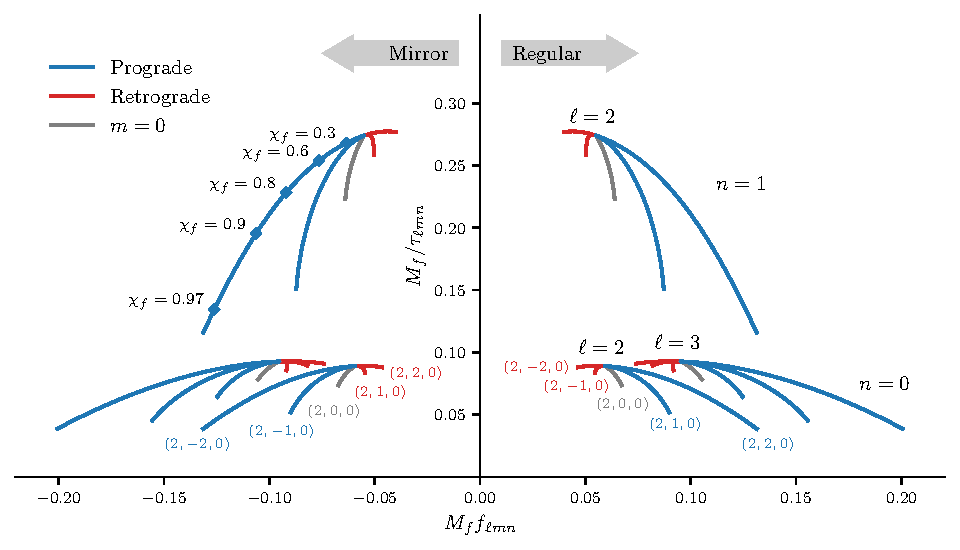
\includegraphics[width=0.9\columnwidth]{Introduction/qnm_taxonomy.pdf}
    \caption[Kerr quasinormal-mode spectrum]{ 
    Selected modes of the Kerr QNM spectrum. BH QNM frequencies are conventionally represented as complex numbers, with the real part giving the  angular frequency of the mode and the imaginary part giving (minus) the inverse of the damping time: $\omega_{\ell m n} = 2\pi f_{\ell m n} - i/\tau_{\ell m n}$. Here we plot $f_{\ell m n}$ and $1/\tau_{\ell m n}$, each scaled by the remnant BH mass $M_f$ to make a dimensionless quantity. The spectrum of a Kerr BH also depends on the dimensionless BH spin magnitude, $\chi_f$; as the spin is increased from zero, branches with different $m$ grow from the points of the Schwarzschild spectrum.
    }
    \label{ch1:fig:qnm_taxonomy}
\end{figure}

We can, alternatively, split the spectrum into ``prograde'' and ``retrograde'' modes. 
This description has the advantage of having a clear physical interpretation; prograde (retrograde) modes are those that are corotating (counterrotating) with the final BH spin.
This can also be expressed as prograde modes satisfying $\mathrm{sgn}\qty(\Re[\omega_{\ell m n}]) = \mathrm{sgn}\qty(m)$, and retrograde modes satisfying $\mathrm{sgn}\qty(\Re[\omega_{\ell m n}]) = -\mathrm{sgn}\qty(m)$.
For binaries where the individual BHs have low spin (or aligned spins that rotate in the same sense as the orbit) it is also expected that the retrograde modes will be suppressed compared to the prograde modes, which is simply a result of the geometry of merger (this has also been shown by studies of numerical simulations, for example in Refs.~\cite{Berti:2005ys, London:2014cma, JimenezForteza:2020cve}).
This assumption is less clear for precessing systems, and is investigated in Chapter~\ref{Chapter2}.
Note that this way of classifying the modes breaks down for $m=0$, leading to some ambiguity. 
This isn't a problem in current data analysis, which focuses on prograde $\ell = \abs{m}$ modes, but since we also perform fits to numerical simulations in this thesis we opt to use the regular-mirror classification.

In terms of spherical harmonics it is known the $\ell=|m|=2$ family of modes dominate the GW strain, and so we expect the same in the ringdown.
Since the overtones decay more quickly (i.e.\ $\tau$ decreases) with increasing $n$, at late times the signal will be dominated by the fundamental $n=0$ modes. 
Therefore, the most prominent QNM in the ringdown is expected to be the $(2,\pm 2,0)$ prograde mode; the observational challenge is usually to detect the presence of other, subdominant modes.

As previously mentioned, the remnant Kerr BH is fully described by only a final mass and a dimensionless final spin~\cite{Carter:1971zc}.
We now denote these quantities $M_f$ and $\chi_f = \abs{\vb*{\chi}_f}$, where the $f$ denotes ``final'' to avoid confusion with the binary properties.
Consequently, the Kerr QNM spectrum is also a function of only the remnant mass and spin.
In Fig.~\ref{ch1:fig:qnm_taxonomy} we can see the mass enters as a scaling on the axes, and the spin gives the position along each branch (we show select spin values along the $(2,-2,1)$ mirror-mode branch).
The Schwarzschild spectrum, which depends only on the BH mass and has no $m$ dependence, can be recovered by taking the branch point of each $(\ell, n)$ group.

This property of Kerr BHs (that they are described by only two parameters in GR) is known as the no-hair theorem, and provides various opportunities for testing GR.
For example, consistency tests can be performed between the inspiral and ringdown~\cite{Hughes:2004vw, Nakano:2015uja, Ghosh:2016qgn, Ghosh:2017gfp}; this involves estimating the remnant properties from an inspiral-only analysis, and separately from a ringdown-only analysis.
In the case of the ringdown, the remnant properties are given directly.
For the inspiral, the binary properties must be projected forward using knowledge from NR simulations (see, for example, Ref.~\cite{Varma:2018aht}).
This test can be posed in an alternative way by using the BH areas; Hawking's area theorem states that the total (classical) BH horizon area cannot decrease over time~\cite{Hawking:1971tu}.
Put another way, in a BBH merger, the total area of the two initial BHs must be smaller than the area of the remnant. 
As the BH area is a simple function of the mass and spin, this test offers an alternative way of testing consistency between measurements of the inspiral and merger (and it does not rely on projecting inspiral parameters forward to merger).
See Refs.~\cite{Cabero:2017avf, Isi:2020tac} for examples of applying this test.

Additionally, we can test the no-hair theorem directly; by simply measuring the QNM frequencies in a ringdown signal we can perform BH spectroscopy.
In analogy with using spectral lines to identify atomic elements, in BH spectroscopy we use the QNM frequencies to identify BHs and their properties.
Initial studies by Echeverria~\cite{Echeverria:1989hg} and Finn~\cite{Finn:1992wt} considered the precision with which the mass and spin of the remnant BH could be measured with a single QNM.
It was in a work by Dreyer et al.~\cite{Dreyer:2003bv} that the importance of measuring multiple QNMs was emphasised, since this leads to tests of the Kerr metric in GR (discussed further below).
This multimode formalism was developed significantly by Berti et al.~\cite{Berti:2005ys, Berti:2007zu}, and there have since been multiple studies on alternative test methods~\cite{Kamaretsos:2011um, Gossan:2011ha}, combining events to place tighter constraints~\cite{Meidam:2014jpa, Yang:2017zxs, DaSilvaCosta:2017njq, Carullo:2018sfu}, and BH spectroscopy prospects with current and future GW detectors~\cite{Berti:2016lat, Bhagwat:2016ntk, Maselli:2017kvl, Baibhav:2018rfk, Bhagwat:2019bwv, Cabero:2019zyt}.

 \begin{figure}[t]
    \centering
    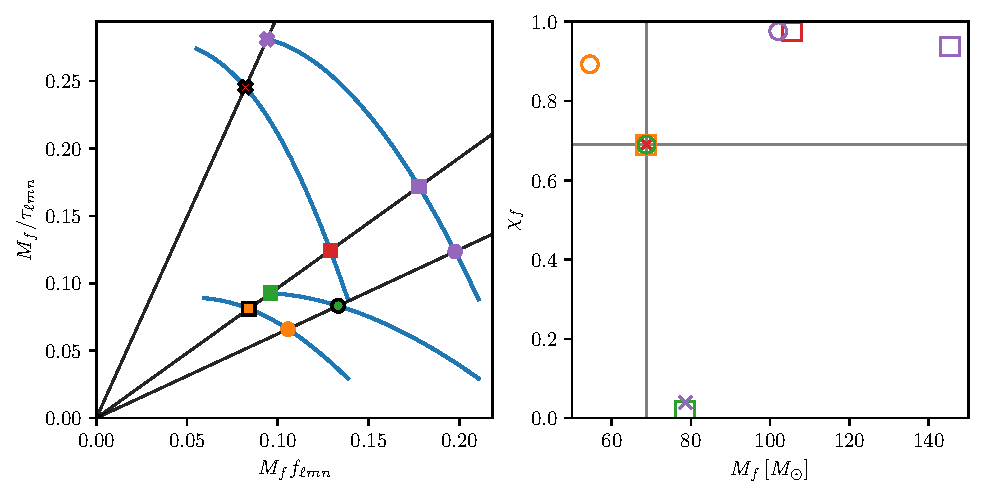
\includegraphics[width=0.9\columnwidth]{Figures/Introduction/bh_spectroscopy.pdf}
    \caption[Black-hole spectroscopy illustration]{
    BH spectroscopy (inspired by a similar figure in Ref.~\cite{Dreyer:2003bv}): a frequency -- damping-time measurement corresponds to a straight line in the left panel. Three such measurements are shown, and their intersections with the Kerr spectrum are indicated. Each measurement is associated with a particular marker shape, and each Kerr branch is associated with a particular marker colour. Each intersection can be converted to a remnant BH mass and spin, shown on the right panel. Only one mass and spin is consistent with all three measurements; these are the true BH properties.
    }
    \label{ch1:fig:bh_spectroscopy}
\end{figure}

Fig.~\ref{ch1:fig:bh_spectroscopy} (inspired by a similar figure in Ref.~\cite{Dreyer:2003bv}) demonstrates the idea behind BH spectroscopy.
On the left panel we show four branches of the Kerr spectrum; the $(2,2,0)$, $(2,2,1)$, $(3,3,0)$ and $(3,3,1)$ modes.
The $(2,2,1)$ and $(3,3,0)$ modes are promising targets for a QNM measurement beyond the fundamental mode, and currently they are the only modes for which there is possible evidence in GW observations~\cite{Isi:2019aib, Capano:2021etf} (these claims are, however, disputed; see Chapters~\ref{Chapter3} and \ref{Chapter4} for further discussion).
In BH spectroscopy, we imagine directly measuring a frequency and damping time in the GW data; say, $f_*$ and $\tau_*$.
In the $M_f f_{\ell m n}$ -- $M_f/\tau_{\ell m n}$ space, this measurement corresponds to a straight line intersecting with the origin; this simply comes from the fact that our scale is not fixed, since we express everything in terms of $M_f$. 
Fixing the value of $M_f$ would collapse the line to a single point, $(f_*,\tau_*)$.
The gradient of the line is given by
\begin{equation}
    \frac{1}{f_* \tau_*} = \frac{\pi}{Q_*},
\end{equation}
where $Q_* = \pi f_* \tau_*$ is the quality factor of the measured mode.
We show three such measurements, and mark where they intersect the Kerr spectrum.
Each intersection corresponds to a particular remnant BH mass, $M_f$, and spin, $\chi_f$. 
The distance of the intersection along the Kerr branch gives the spin.
The mass is found by, for example, dividing the value of $M_f f_{\ell m n}$ at the intersection by the measured frequency $f_*$.
Since each measurement line will generically intersect with multiple Kerr branches, they return multiple $(M_f, \chi_f)$ values. 
However, assuming the BH is indeed described by the Kerr metric, then there will be a single $(M_f,\chi_f)$ combination consistent with all the measurements (indicated by the horizontal and vertical lines in the right panel).
If no such combination exists, then what is observed is either not an isolated BH, or it is not described by the Kerr metric in GR. 

The above describes the key idea behind BH spectroscopy, but in practice the test is performed slightly differently.
Firstly, in reality it may not be practical to measure multiple QNM frequencies directly due to parameter degeneracies that come with summing functionally equivalent QNMs.
And secondly, it can be tricky to turn multiple frequency--damping-time measurements into a quantitative statement regarding compatibility with the GR Kerr spectrum.
Instead, we can target the loudest QNMs in the data and parameterise all the QNM frequencies with a single mass and spin (according to the Kerr spectrum).
That is,
\begin{equation}
    \omega_{\ell m n} = \omega_{\ell m n}(M_f, \chi_f).
\end{equation}
This reduces the dimensions of the problem, and also directly measures the physically relevant properties of the remnant BH.
With the expectation that what we measure will not be greatly different from the GR Kerr prediction, we can measure any disagreement by allowing a subset of the QNMs in our model to deviate from Kerr in the following way:
\begin{equation}
    f = f_{\ell m n}(M_f, \chi_f) e^{\delta f_{\ell m n}} \qquad \tau = \tau_{\ell m n}(M_f, \chi_f) e^{\delta \tau_{\ell m n}}.
\end{equation}
We emphasise that not all the modes in the model should be allowed to vary, since then the analysis becomes equivalent to a direct search of frequencies and damping times.
The new parameters, $\delta f_{\ell m n}$ and $\delta \tau_{\ell m n}$, will have measurements consistent with zero if the data is well described by Kerr.
Additionally, the uncertainty on the measurements of the $\delta$ parameters give us a natural test confidence. 
This method of testing the no-hair theorem is described further in Ref.~\cite{Isi:2021iql}, and is employed in Section~\ref{subsec:verify} for our analysis of GW150914.
